\documentclass[11pt,a4paper]{article}
\usepackage[T1]{fontenc}
\usepackage[utf8]{inputenc}
\usepackage{lmodern}
\usepackage[a4paper,margin=2.55cm]{geometry}
\usepackage{amsmath,amssymb}
\usepackage{graphicx}
\usepackage{booktabs}
\usepackage[font=small,labelfont=bf]{caption}
\usepackage{xurl}
\usepackage[hidelinks]{hyperref}
\graphicspath{{images/}}
\pdfminorversion=7

\newcommand{\reporttitle}{Optimizing effective inertia at collision point\\to minimize energy transfer -- Franka Emika}
\newcommand{\reportdegree}{Robotics II}
\newcommand{\academicyear}{2025/2026}
\newcommand{\Jm}{J_M^{\#}}
\newcommand{\ms}{m_n^-}
\newcommand{\vs}{v_n^-}
\newcommand{\diag}{\operatorname{diag}}

\begin{document}
% Sapienza Universita di Roma -- title page (DIAG)
% Edit title, degree, date and academic year in main.tex.
\begin{titlepage}
  \centering
  \vspace*{-0.6cm}
  
\includegraphics[width=0.48\textwidth]{sapienza_logo}\par
  \vspace{1.9cm}
  {\large\scshape Department of Computer, Control and Management\\ Engineering\par}
  \vspace{3.4cm}
  {\LARGE\bfseries \reporttitle\par}
  \vspace{0.9cm}
  {\Large\scshape \reportdegree\par}
  \vspace{0.6cm}
  {\normalsize \reportdate\par}
  \vspace{2.4cm}
  \begin{minipage}[t]{0.42\textwidth}
    \raggedright
    {\large\bfseries Professor:\par}\vspace{0.35cm}
    Alessandro De Luca\par\vspace{0.6cm}
    {\large\bfseries Co-supervisor:\par}\vspace{0.35cm}
    Mattia Castelmare
  \end{minipage}%
  \begin{minipage}[t]{0.38\textwidth}
    \raggedright
    {\large\bfseries Students:\par}\vspace{0.35cm}
    Lorenzo Carlino\\
    Samuele Leonardi\\
    Gurwinder Sharma
  \end{minipage}
  \vfill
  \rule{\textwidth}{0.6pt}\par
  \vspace{0.6cm}
  Academic Year \academicyear\par
  \vspace{2.3cm}
\end{titlepage}

\setcounter{page}{1}
\tableofcontents
\clearpage

\section{Project objective}
The project studies how the seven-joint Franka Emika R3 can change its posture
to reduce the directional effective mass at a known point of collision.
The robot follows a Cartesian position trajectory toward a compliant wall.
Its redundant motion provides freedom to change the inertia reflected at
the fingertip while preserving the requested tracking task.

We compare two control laws. The baseline uses inverse dynamics and a
Jacobian pseudoinverse for Cartesian tracking, together with posture feedback.
The optimized law uses a single quadratic program (QP) that balances Cartesian
tracking with a joint acceleration preference for lower effective mass. Both
laws are applied to a circular trajectory and to a perpendicular approach.

The quantitative target is at least a 30\% reduction in effective mass
immediately before the first impact, relative to the corresponding baseline.
The comparisons keep the reference trajectory, contact model and Cartesian
feedback gains equal within each pair. Normal velocity, contact loads and
tracking error are evaluated together to assess the effect of the changed
posture. The momentum observer estimates the external joint torques, from which the normal contact force is reconstructed.

\section{Robot dynamics, contact and effective mass}
\subsection{Rigid-body model and torque convention}
Let $q,\dot q,\ddot q\in\mathbb R^7$ be the joint position, velocity and
acceleration. The nominal rigid-body dynamics are
\begin{equation}
 M(q)\ddot q+C(q,\dot q)\dot q+g(q)
 =\tau_a+\tau_{\mathrm{ext}},
 \label{eq:dynamics}
\end{equation}
where $M$ is the positive-definite joint inertia matrix, $C\dot q$ contains
Coriolis and centrifugal terms, $g$ is the gravity torque, $\tau_a$ is the
motor torque, and $\tau_{\mathrm{ext}}$ is the torque caused by external contact.
We use $c(q,\dot q)=C(q,\dot q)\dot q$ below.

In the Gazebo setup used in this project, gravity compensation is automatically provided by the Franka simulation plugin. If
$\tau_c$ is the additional torque applied after command clipping and transport,
then $\tau_a=g(q)+\tau_c$. The resulting dynamics are
\begin{equation}
 M\ddot q+c=\tau_c+\tau_{\mathrm{ext}}.
 \label{eq:compensated}
\end{equation}
The gravity term $g$ is included in the formulation of the full
motor-torque control laws, while only the gravity-compensated component
is passed to the software.

The fingertip position is $p(q)\in\mathbb R^3$, expressed in the fixed robot
base frame. Its translational Jacobian is
\begin{equation}
 J(q)=\frac{\partial p}{\partial q}\in\mathbb R^{3\times7},
 \qquad \dot p=J\dot q,\qquad
 \ddot p=J\ddot q+\dot J\dot q .
 \label{eq:kinematics}
\end{equation}
The position task has four redundant degrees of freedom when $J$ has full
row rank. The formulations below assume that rank condition.

\subsection{Virtual wall and force direction}
The wall is a plane through $p_w$, with unit outward normal $n$. The signed
penetration and the normal velocity toward the wall are
\begin{equation}
 \delta=n^{\mathsf T}(p_w-p),\qquad v_n=-n^{\mathsf T}J\dot q .
\end{equation}
Positive $\delta$ places the fingertip inside the wall. The virtual contact law is
\begin{equation}
 F_n=
 \begin{cases}
 \max\!\bigl(0,k_e\delta+b_e\max(v_n,0)\bigr),&\delta>0,\\
 0,&\delta\le0,
 \end{cases}
 \qquad F=F_n n,\qquad \tau_{\mathrm{ext}}=J^{\mathsf T}F .
 \label{eq:wall}
\end{equation}
Here $k_e$ is wall stiffness and $b_e$ is damping, active during compression.
The force acts only at the fingertip. The simulator records $F_n$ as a
reference for evaluating the impact and the observer.

\subsection{Directional effective mass}
The Cartesian inertia and effective mass along $n$ are
\begin{equation}
 \Lambda(q)=\bigl(JM^{-1}J^{\mathsf T}\bigr)^{-1},\qquad
 m_n(q)=\frac{1}{n^{\mathsf T}JM^{-1}J^{\mathsf T}n}.
 \label{eq:mass}
\end{equation}
The scalar $m_n$ describes the instantaneous inertial response at the
fingertip in the chosen direction. Redundancy changes $m_n$ through $q$.
The physical mass of the robot is constant.
For a force $F_n n$ at a fixed configuration, its contribution to normal
Cartesian acceleration is
$n^{\mathsf T}JM^{-1}J^{\mathsf T}nF_n=F_n/m_n$.

The superscript minus denotes the sample immediately before first contact.
The normal equivalent kinetic energy is
\begin{equation}
 E_n^-=\tfrac12\ms(\vs)^2 .
 \label{eq:entry-energy}
\end{equation}
At a given normal velocity, a smaller $\ms$ reduces this inertial contribution
to impact. Equation~\eqref{eq:entry-energy} is a pre-impact metric.
The energy transferred to the environment also depends on the subsequent
force and motion, including the work of the actuators during contact.

\section{Momentum observer and collision detection}
\subsection{External joint-torque estimate}
The generalized momentum is $\pi=M(q)\dot q$. With the convention
$\dot M=C+C^{\mathsf T}$, equation~\eqref{eq:dynamics} gives
\begin{equation}
 \dot\pi=\tau_a-g+C^{\mathsf T}\dot q+\tau_{\mathrm{ext}}.
\end{equation}
The momentum observer~\cite{deluca2005,haddadin2017} integrates
\begin{equation}
 \dot{\widehat\pi}=\tau_a-g+C^{\mathsf T}\dot q+r,
 \qquad r=K_O(\pi-\widehat\pi),\qquad K_O>0\text{ diagonal}.
 \label{eq:observer}
\end{equation}
At the first observer sample $t_0$, the initialization
$\widehat\pi(t_0)=\pi(t_0)$ gives $r(t_0)=0$.
The observer uses measured joint states and the applied actuator torque.
In the gravity-compensated implementation, $\tau_a-g$ is reconstructed
from the delayed, clipped command history averaged over each sample interval.
The simulated wall torque is excluded from that input.

Under the nominal model, the residual obeys
\begin{equation}
 \dot r=K_O(\tau_{\mathrm{ext}}-r).
 \label{eq:residual-filter}
\end{equation}
Thus $r$ is a filtered estimate of the external joint torque, measured in
N\,m. The time constant of component $i$ is $1/K_{O,ii}$. A faster observer
can detect rapid changes sooner but is more sensitive
to measurement errors, model inaccuracies and torque delays.

\subsection{Collision detection}
Contact is detected when at least one component of the residual exceeds
its corresponding joint-torque threshold $\theta_i$, that is,
\begin{equation}
 \exists i\in\{1,\ldots,7\}\quad |r_i|>\theta_i ,
 \label{eq:detector}
\end{equation}
A detection event occurs when this condition becomes true. The indices
of the residual components that exceed their thresholds indicate which
joints triggered the detection. However, they are not used to locate
the contact, which is assumed to occur at the fingertip.

The runner uses the observer for collision monitoring and records the
residual for offline force reconstruction. Both controllers compute their
commands from the measured joint state and the reference. The detection
flag and reconstructed force are used for analysis.

\subsection{Offline contact-force reconstruction}
The reconstruction assumes one active contact point at a time, located
at the fingertip, with force acting along the known wall normal $n$.
It is evaluated throughout the recorded run and applies to all
successive impacts and recontacts.

The observer is integrated using implicit Euler. We invert its discrete
filter using the recorded gain and sample interval
$\Delta t_k=t_k-t_{k-1}$
\begin{equation}
 \widetilde\tau_{\mathrm{ext},k}
 =r_k+K_O^{-1}\frac{r_k-r_{k-1}}{\Delta t_k},\qquad
 h_k=J(q_k)^{\mathsf T}n,\qquad
 \widehat F_{n,k}
 =\frac{h_k^{\mathsf T}\widetilde\tau_{\mathrm{ext},k}}
        {h_k^{\mathsf T}h_k}.
 \label{eq:force-estimation}
\end{equation}
The last expression chooses the normal force $\widehat F_{n,k}$ whose
joint-torque contribution, $h_k\widehat F_{n,k}$, best matches the
reconstructed external torque. This requires
$h_k^{\mathsf T}h_k>0$, meaning that a force in the assumed direction
produces a measurable effect on the joints. The correction starts at
the second sample because it uses two consecutive residuals.

Using $r_k$ directly retains the smoothing and delay introduced by the
observer. Filter inversion compensates for these effects by including
the rate of change of the residual. This improves the reconstruction
of short force peaks under nominal conditions, while increasing
sensitivity to noise and timing errors.

The force is reconstructed offline from the recorded residuals and
joint positions. Collision detection uses the filtered residual from
equation~\eqref{eq:observer}.

\section{Control laws}
\subsection{Baseline Cartesian tracking}
Let $p_d(t)$, $v_d(t)$ and $a_d(t)$ be the desired Cartesian position, velocity
and acceleration. Define
\begin{equation}
 e=p_d-p,\qquad \dot e=v_d-J\dot q,\qquad
 b=a_d+K_p e+K_d\dot e-\dot J\dot q ,
 \label{eq:tracking-target}
\end{equation}
with diagonal position and derivative feedback gains
$K_p,K_d\in\mathbb R^{3\times3}$ having positive entries.
This is proportional--derivative (PD) feedback at acceleration level with
feedforward acceleration.

For the baseline, the Euclidean pseudoinverse and null-space projector are
$J^\dagger=J^{\mathsf T}(JJ^{\mathsf T})^{-1}$ and $N_E=I-J^\dagger J$.
The complete requested motor-torque law is
\begin{equation}
 \boxed{\begin{aligned}
 u_B&=J^\dagger b+
        N_E\bigl[k_{q,B}(q_0-q)-k_{\mathrm{ns},B}\dot q\bigr],\\
 \tau_{a,B}^{\mathrm{des}}&=M(q)u_B+c(q,\dot q)+g(q).
 \end{aligned}}
 \label{eq:baseline}
\end{equation}
Here $q_0$ is the initial joint configuration, $k_{q,B}>0$ is a posture gain,
and $k_{\mathrm{ns},B}>0$ damps redundant joint motion. The initial posture attraction discourages accumulated motion away from the starting posture.

Since gravity compensation is handled separately by the simulator,
the software computes the actuator command as
$\tau_{a,B}^{\mathrm{des}}-g=Mu_B+c$. Before the command is sent to
the actuators, each torque component is checked against its permitted
range and saturated if necessary.

Under nominal conditions, assuming an exact model, negligible delays
and no torque saturation, the controller achieves the desired Cartesian
error dynamics
\begin{equation}
 \ddot e+K_d\dot e+K_p e=0.
 \label{eq:nominal-error}
\end{equation}
The convergence of the position and velocity errors is therefore
governed by the feedback gains $K_p$ and $K_d$. When contact occurs,
however, the external torque introduces an additional acceleration
term $M^{-1}\tau_{\mathrm{ext}}$ at the joint level, causing the robot
to deviate from its nominal tracking behavior.

\subsection{Online effective mass reduction}

The optimized controller follows the same Cartesian tracking target $b$
introduced in equation~\eqref{eq:tracking-target}, while exploiting the
kinematic redundancy of the robot to reduce its effective mass.
To this end, a preferred joint acceleration is computed by combining
Cartesian tracking, null-space damping and effective mass optimization.
The QP uses this preference alongside the Cartesian tracking target
when selecting an actuator command subject to joint braking and torque bounds.

To introduce secondary objectives without interfering with Cartesian
tracking, the controller uses the mass-weighted pseudoinverse and the
associated null-space projector, defined as
\begin{equation}
 \Jm=M^{-1}J^{\mathsf T}(JM^{-1}J^{\mathsf T})^{-1},
 \qquad N_M=I-\Jm J .
 \label{eq:weighted-inverse}
\end{equation}
Among all joint accelerations satisfying $Ju=b$, the solution
$\Jm b$ minimizes the mass-weighted quadratic cost
$\tfrac12u^{\mathsf T}Mu$. Moreover, the properties $JN_M=0$ and
$JM^{-1}N_M^{\mathsf T}=0$ allow additional acceleration and torque
contributions to be introduced in the null space without affecting
the nominal Cartesian tracking task~\cite{khatib1987}.

The effective mass optimization is based on the gradient
$\nabla_q m_n(q)$, which describes how the effective mass along
direction $n$ varies with the joint configuration. This gradient is
computed analytically at the current configuration. By introducing
$j=J^{\mathsf T}n$ and $x=M^{-1}j$, the derivative of
equation~\eqref{eq:mass} with respect to each joint coordinate can
be expressed as
\begin{equation}
 \frac{\partial m_n}{\partial q_i}
 =m_n^2\left[
 x^{\mathsf T}\frac{\partial M}{\partial q_i}x
 -2\left(\frac{\partial j}{\partial q_i}\right)^{\mathsf T}x
 \right].
 \label{eq:mass-gradient}
\end{equation}

The idea is to guide the robot toward configurations characterized
by a lower effective mass by introducing a torque contribution
along the negative direction of the gradient. This torque is
projected into the dynamic null space, giving no nominal Cartesian
acceleration at the current configuration. The resulting
torque $\tau_m$ and preferred joint acceleration $u_{\mathrm{pref}}$
are given by
\begin{equation}
 \boxed{\begin{aligned}
 \tau_m&=-\alpha(t)k_m N_M^{\mathsf T}\nabla_qm_n(q),\\
 u_{\mathrm{pref}}&=\Jm b-k_{\mathrm{ns}}N_M\dot q
       +\beta(t)k_{q,R}N_M(q_0-q)+M^{-1}\tau_m .
 \end{aligned}}
 \label{eq:preference}
\end{equation}
The gain $k_m>0$ determines the contribution of the effective mass
gradient, while $k_{\mathrm{ns}}>0$ provides damping for redundant
joint motion. Since the optimization is formulated as a torque
contribution, multiplication by $M^{-1}$ is required to express it
in terms of joint acceleration.

The coefficients $\alpha(t)$ and $\beta(t)$ allow the controller
to smoothly change its secondary objective during the different
phases of motion. During tracking, $\beta=0$, while $\alpha\in[0,1]$
gradually activates effective mass optimization. During the circular
return, the effective mass contribution is progressively reduced
through $\alpha$, while $\beta\in[0,1]$ gradually activates posture
feedback toward the initial configuration $q_0$, with gain $k_{q,R}$.


The approach is referred to as \emph{full online} effective mass
optimization because the gradient is continuously evaluated during
motion, rather than relying on a contact posture computed through
an offline optimization procedure. In this way, the controller
can adapt the robot configuration as the Cartesian trajectory
is followed.

The QP selects $u_{\mathrm{sel}}$ by weighing the Cartesian error and
the deviation from $u_{\mathrm{pref}}$ under the constraints in
Section~\ref{sec:qp}. The corresponding desired motor torque is
obtained through inverse dynamics as
\begin{equation}
 \boxed{\tau_{a,Q}^{\mathrm{des}}
 =M(q)u_{\mathrm{sel}}+c(q,\dot q)+g(q).}
 \label{eq:optimized-output}
\end{equation}

\section{Constrained quadratic program}
\label{sec:qp}
\subsection{Decision variable and objective}
At each update the controller evaluates the robot model at the measured
$(q,\dot q)$. The decision variable is the actuator-induced acceleration
\begin{equation}
 u=M^{-1}(\tau_{\mathrm{cmd}}-c)\in\mathbb R^7,
 \label{eq:qp-variable}
\end{equation}
where $\tau_{\mathrm{cmd}}$ is the gravity-compensated command. With that
command applied and the nominal dynamics, the actual acceleration is
$\ddot q=u+M^{-1}\tau_{\mathrm{ext}}$.

The controller selects $u_{\mathrm{sel}}$ by solving
\begin{equation}
 \boxed{\begin{aligned}
 \underset{u}{\operatorname{minimize}}\quad&
 \tfrac{w}{2}\|Ju-b\|^2+\tfrac12\|u-u_{\mathrm{pref}}\|^2\\
 \text{subject to}\quad&
 \underline u\le u\le\overline u,\qquad
 |Mu+c+\tfrac12g|\le T-\tfrac12|g|.
 \end{aligned}}
 \label{eq:single-qp}
\end{equation}
The first term penalizes Cartesian tracking error at the acceleration
level. The second favors the joint acceleration from
equation~\eqref{eq:preference}, which contains damping, the mass gradient
and, during circular RETURN, posture feedback. The weight $w$ favors
tracking when limits are active. If $u_{\mathrm{pref}}$ is feasible, then
$Ju_{\mathrm{pref}}=b$ and both costs attain their minimum at that
preference. When the bounds are active, the finite weight allows a
trade-off between tracking and the joint preference.

\subsection{Joint braking bounds and torque limits}
Let $Q_{\min},Q_{\max}$ be the physical joint position limits, $V$ the
joint speed limits and $T$ the actuator torque limits. The braking
interval is inset by a position margin $m_h$ and an additional buffer
$m_b$. Its lower and upper distances from the current state are
\begin{equation}
 d_\ell=q-(Q_{\min}+m_h+m_b),\qquad
 d_u=(Q_{\max}-m_h-m_b)-q .
\end{equation}
The allowed outward speed decreases with the remaining travel.
For either distance $d$, the position constraint uses
$s=\dot d+\kappa_q d$ and imposes $\dot s+\kappa_v s\ge0$ under the
nominal acceleration $u$. The speed constraints use the same rate
$\kappa_v$ on the distances $V+\dot q$ and $V-\dot q$ from the speed
limits. Combining these inequalities gives the componentwise bounds
\begin{equation}
 \begin{aligned}
 \underline u&=\max\bigl\{
 -(\kappa_q+\kappa_v)\dot q-\kappa_q\kappa_v d_\ell,\quad
 -\kappa_v(V+\dot q)\bigr\},\\
 \overline u&=\min\bigl\{
 -(\kappa_q+\kappa_v)\dot q+\kappa_q\kappa_v d_u,\quad
 \kappa_v(V-\dot q)\bigr\}.
 \end{aligned}
 \label{eq:braking-bounds}
\end{equation}
The buffer starts circular joint braking earlier near the end of joint
travel. These inequalities bound the nominal actuator acceleration
using the current measurements. Wall force can change the actual
joint acceleration and carry a joint into the buffer.

The torque inequality in equation~\eqref{eq:single-qp} represents the
intersection of the published command limit $|\tau_{\mathrm{cmd}}|\le T$
and the nominal motor limit $|\tau_{\mathrm{cmd}}+g|\le T$, where
$\tau_{\mathrm{cmd}}=Mu+c$. The QP enforces all these inequalities as hard
constraints.

\subsection{Numerical implementation and command selection}
The Hessian is $wJ^{\mathsf T}J+I$ and the linear term is
$-wJ^{\mathsf T}b-u_{\mathrm{pref}}$. The Hessian is positive definite,
giving a unique optimum when the constraints are feasible. The
operator-splitting solver OSQP retains the matrix sparsity pattern and
warm-starts from its previous solution. The controller verifies the available
solution against the original inequalities before publishing the
command. A solve with no accepted solution ends the trial with bounded
joint damping, provided the two torque ranges still intersect.

\section{Repeated motion and reference transitions}
\label{sec:return}
The perpendicular reference completes one approach and an endpoint hold.
For both control laws, collision detection leaves this reference active.
The online secondary preference continues during contact.

Repeated circular motion requires an additional posture policy. Early
full-online runs accumulated changes in joint posture and hand orientation
from lap to lap. We therefore return physically to $q_0$ after each revolution.
The baseline uses the same schedule so that later approaches occur at
matching times.

Each circular cycle has a tracking phase followed by RETURN. A quintic
Cartesian braking reference starts from the position, velocity and
acceleration at the lap boundary and ends at $p(q_0)$ with zero velocity
and acceleration. The reference then holds that point while the redundant
joints approach $q_0$.

The smoothstep $\sigma(s)=3s^2-2s^3$, with $s$ clipped to $[0,1]$, controls
the online preferences. At the start of each tracking phase, $\alpha$ rises
from zero to one and $\beta=0$ in equation~\eqref{eq:preference}.
During the braking transition, $\alpha$ falls from one to zero, $\beta$
rises from zero to one, and damping blends to
$k_{\mathrm{ns}}=2\sqrt{k_{q,R}}$. On later restarts it blends back to
the tracking value. The baseline retains its own posture and damping terms.

RETURN has a fixed duration shared by the two laws. A new lap begins at
the scheduled time only if the maximum joint position error and speed
are within the restart tolerances. Otherwise the trial terminates.
The observer continues using absolute run time through every transition.

\clearpage
\section{Simulation setup and evaluation}
\subsection{Plant, contact and timing}
Gazebo simulates the robot and receives torque commands. The Pinocchio
library provides the kinematic and dynamic model from the same robot
description, including reflected rotor inertia. All reported comparisons
use nominal inertial parameters with joint friction and measurement noise
disabled.

The initial joint configuration and fingertip position are
\begin{equation}
 q_0=[0,-0.1517,0,-2.6105,0,4.0295,0.785]^{\mathsf T}\ \mathrm{rad},
 \qquad p(q_0)\simeq(0.56,0,0.50)\ \mathrm m .
\end{equation}
In equation~\eqref{eq:wall}, the wall uses
$p_w=(0.62,0,0.50)$\,m, $n=(-1,0,0)^{\mathsf T}$,
$k_e=20\,000$\,N/m and $b_e=15$\,N\,s/m.

The control rate is 1000\,Hz in simulation time. The real-time factor (RTF)
is simulated elapsed time divided by wall-clock elapsed time. At the
requested RTF of 0.20, one simulated second takes approximately five
wall-clock seconds, giving about 5\,ms for each simulated 1\,ms step.
Slowing the simulation allows a computation longer than 1\,ms to finish
before the next sample.
The observer is enabled in all four reported trials for collision monitoring
and offline force reconstruction.

The circular reference lies in the $x$--$z$ plane, has radius 0.04\,m, and
starts at the leftmost point of the circle. Its centre is
$p(q_0)+(0.04,0,0)$\,m. The cruise period is 2\,s, with a 1\,s smooth ramp
in angular velocity. Integrating the ramp makes each revolution last
2.5\,s. Every lap restarts the ramp. Each cycle follows
\[
 \underbrace{\mathrm{TRACK}}_{2.5\,\mathrm{s}}
 \longrightarrow
 \underbrace{\mathrm{BRAKING}}_{0.20\,\mathrm{s}}
 \longrightarrow
 \underbrace{\text{hold }p(q_0)\text{ and return to }q_0}_{1.80\,\mathrm{s}}
 \longrightarrow
 \text{restart check}.
\]
BRAKING and the subsequent hold make up the 2.0\,s RETURN phase.
The restart check requires every joint error to be at most 0.001\,rad
and every joint speed to be at most 0.005\,rad/s. Each run lasts 20\,s.

The perpendicular reference accelerates to 0.20\,m/s over 0.10\,s, follows
the wall normal, and brakes over its final 4\,mm. Its endpoint is 10\,mm
beyond the wall plane and is held for 0.15\,s. That endpoint specifies
desired position. Actual penetration follows equation~\eqref{eq:wall}
and the controlled robot dynamics. Both selected trials complete at about
0.57\,s, within the 2\,s launch limit.

\subsection{Gains and constraint parameters}
\begin{center}
\begin{tabular}{lll}
\toprule
Parameter & Value & Meaning\\
\midrule
$K_p,\ K_d$ & $100I_3,\ 20I_3$ & Cartesian PD gains, s$^{-2}$ and s$^{-1}$\\
$k_{q,B},\ k_{\mathrm{ns},B}$ & $25,\ 10$ & Baseline posture and damping\\
$k_m,\ k_{\mathrm{ns}}$ circular & $2,\ 24$ & Online gradient and damping\\
$k_m,\ k_{\mathrm{ns}}$ perpendicular & $4,\ 12$ & Online gradient and damping\\
$k_{q,R},\ k_{\mathrm{ns}}$ in RETURN & $25,\ 10$ & Online return posture and damping\\
$w$ & $1000$ & Cartesian tracking weight in the QP\\
$\kappa_q,\ \kappa_v$ & $6,\ 60$ & Joint braking rates, s$^{-1}$\\
$K_O,\ \theta_i$ & $30I_7,\ 0.1$ & Observer gain s$^{-1}$ and threshold N\,m\\
\bottomrule
\end{tabular}
\end{center}
The units of $k_q$, $k_{\mathrm{ns}}$ and $k_m$ are s$^{-2}$, s$^{-1}$
and N\,m\,rad/kg, respectively. The Cartesian gains give critical damping
at 10\,rad/s in equation~\eqref{eq:nominal-error}. The posture gains give
critical damping at 5\,rad/s in a scalar approximation.

The online gains are based on earlier nominal trials. The perpendicular
pair $k_m=4$, $k_{\mathrm{ns}}=12$ was selected to reduce the effective
mass within the short approach time while retaining joint clearance. The
circular pair uses more damping and a smaller mass gain during repeated
tracking. The 0.10\,s mass ramp reaches full activation before the first
impact in both experiments. The QP weight emphasizes Cartesian tracking
when braking bounds or torque limits become active.

The position margin $m_h$ is 0.06\,rad, leaving 0.01\,rad before the
simulation's 0.05\,rad joint-limit stop band. The circular configuration
adds $m_b=0.09$\,rad to the braking distances in
equation~\eqref{eq:braking-bounds}, giving 0.15\,rad of preventive clearance.
The perpendicular configuration uses $m_b=0$. During impact, the measured
motion can enter the circular braking buffer while remaining outside the
hard margin.
The physical position, velocity and torque limits are given in
Table~\ref{tab:joint-limits}.

\begin{table}[htbp]
\centering
\begin{tabular}{rrrrr}
\toprule
Joint & $Q_{\min}$ (rad) & $Q_{\max}$ (rad) & $V$ (rad/s) & $T$ (N\,m)\\
\midrule
1 & $-2.7437$ & $2.7437$ & 2.62 & 87\\
2 & $-1.7837$ & $1.7837$ & 2.62 & 87\\
3 & $-2.9007$ & $2.9007$ & 2.62 & 87\\
4 & $-3.0421$ & $-0.1518$ & 2.62 & 87\\
5 & $-2.8065$ & $2.8065$ & 5.26 & 12\\
6 & $0.5445$ & $4.5169$ & 4.18 & 12\\
7 & $-3.0159$ & $3.0159$ & 5.26 & 12\\
\bottomrule
\end{tabular}
\caption{Joint limits used by the model and motion constraints.}
\label{tab:joint-limits}
\end{table}

OSQP uses absolute and relative tolerances of $10^{-6}$, at most 1000
iterations per solve, termination checks every ten iterations, adaptive
penalty updates and polishing disabled. The independent inequality check
allows a maximum error of $2\times10^{-4}$ in the units of the corresponding
acceleration or torque constraint.

\subsection{Metrics and recorded runs}
The first contact time $t_c$ is the first sample with $F_n>0$.
The first compression--release cycle ends at $t_e$, the first detachment
or the start of recompression, whichever occurs first. Recompression
begins at the zero crossing obtained by linearly interpolating the
first change of $v_n$ from outward to inward motion after release.
Pre-impact effective mass and velocity are taken strictly from the
sample preceding $t_c$.
The normal impulse and pre-impact root mean square (RMS) tracking error are
\begin{equation}
 I_n=\int_{t_c}^{t_e}F_n(t)\,dt,\qquad
 e_{\mathrm{RMS}}=
 \sqrt{\frac{1}{t_--t_s}\int_{t_s}^{t_-}\|p_d(t)-p(t)\|^2\,dt},
 \label{eq:metrics}
\end{equation}
where $t_s$ is the first recorded sample used in the tracking-error
integral and $t_-$ is the last sample before contact. All four runs start
at recorded time $t_s=0$. Integrals use trapezoids at actual sample times.
Constraint checks cover recorded samples.

The two pairs use the single-QP controller runs and their corresponding
baselines recorded on 27 November 2026. Appendix~\ref{app:sources} identifies
the logs. Reported changes are relative to each experiment's baseline, using
full-precision values before rounding.

\clearpage
\section{Simulation results}
\subsection{Circular trajectory}
\begin{table}[htbp]
\centering
\begin{tabular}{lrrr}
\toprule
Metric & Baseline & Full online & Change (\%)\\
\midrule
Contact onset (s) & 1.167 & 1.165 & --\\
Pre-impact effective mass (kg) & 7.189 & 4.607 & $-35.92$\\
Pre-impact normal velocity (m/s) & 0.10893 & 0.10906 & $+0.11$\\
Pre-impact normal energy (mJ) & 42.656 & 27.395 & $-35.78$\\
Peak force (N) & 43.147 & 34.387 & $-20.30$\\
First-cycle impulse (N\,s) & 2.1017 & 1.2624 & $-39.93$\\
Peak penetration (mm) & 2.155 & 1.716 & $-20.38$\\
First-cycle duration (ms) & 84.0 & 59.0 & $-29.76$\\
Pre-impact RMS error (mm) & 0.0190 & 0.2998 & --\\
\bottomrule
\end{tabular}
\caption{First circular compression--release cycle.}
\label{tab:circular}
\end{table}

The online controller reaches a substantially lower effective mass at the
same normal velocity (Table~\ref{tab:circular}). Its peak contact force
drops by about one fifth. The reduction in impulse is larger because
the mean force over the first cycle falls from 25.0 to 21.4\,N and the
cycle is 25\,ms shorter. The RMS tracking error grows by 0.281\,mm.
The nearly equal entry speeds keep the first-impact comparison relevant
despite the change in tracking accuracy.

Figures~\ref{fig:circular-baseline-first} and~\ref{fig:circular-online-first}
show each first impact separately. Both trials complete 20\,s with four
scheduled returns. Successive approaches are 4.5\,s apart in both runs.
The online first contacts occur 2\,ms earlier than their baseline
counterparts, and the recontacts occur 5\,ms earlier. Each run records
ten episodes, all during tracking, as shown in
Figures~\ref{fig:circular-baseline-all} and~\ref{fig:circular-online-all}.

\begin{figure}[p]
\centering
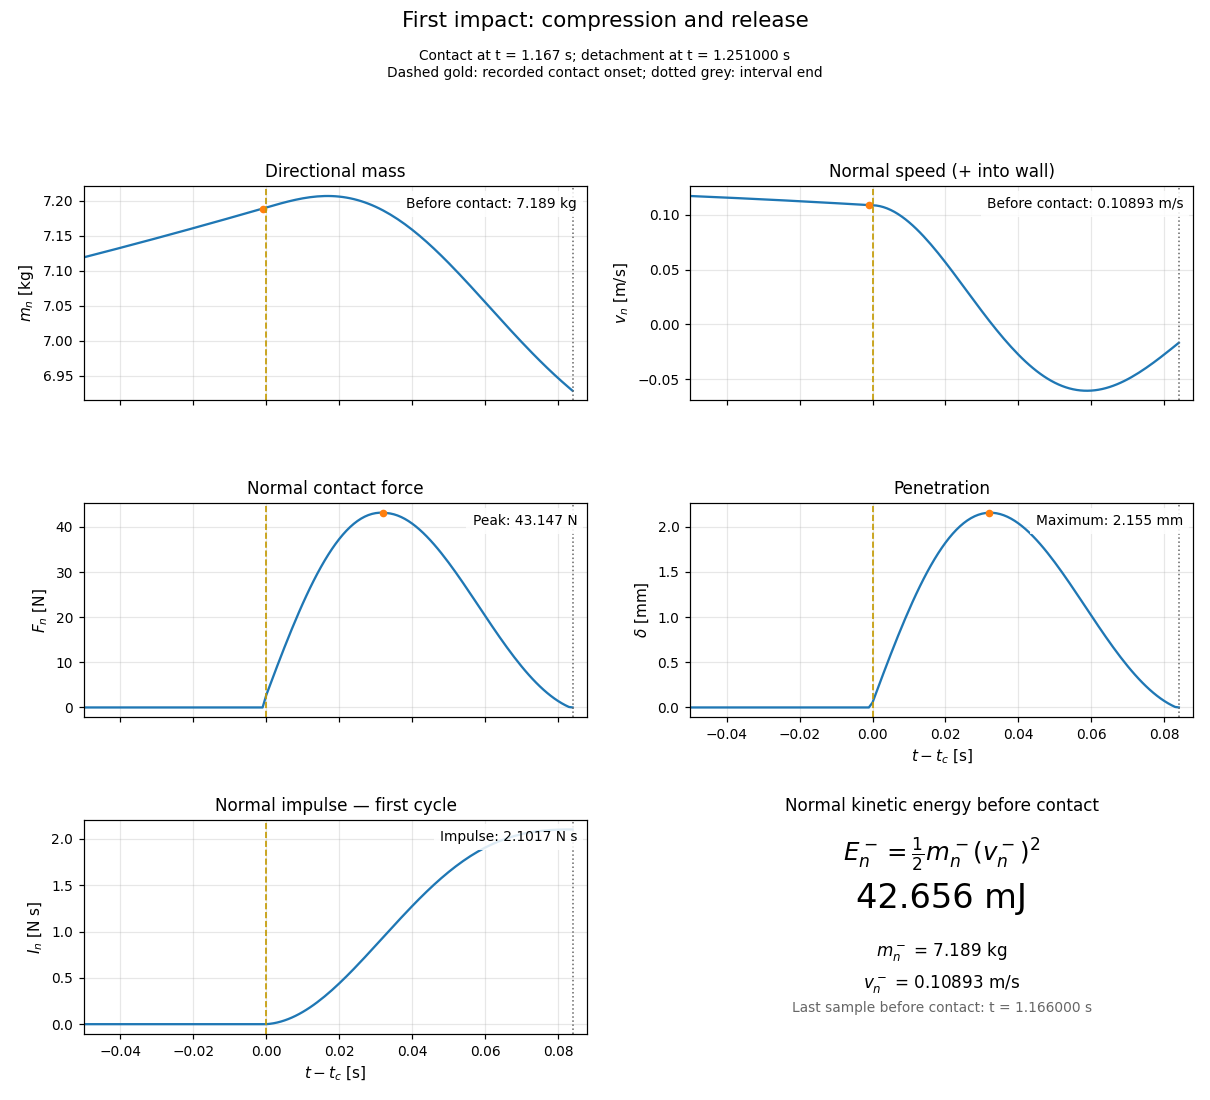
\includegraphics[width=\linewidth]{fig03_circular_baseline_first_impact}
\caption{Circular baseline, first compression--release cycle.}
\label{fig:circular-baseline-first}
\end{figure}
\begin{figure}[p]
\centering
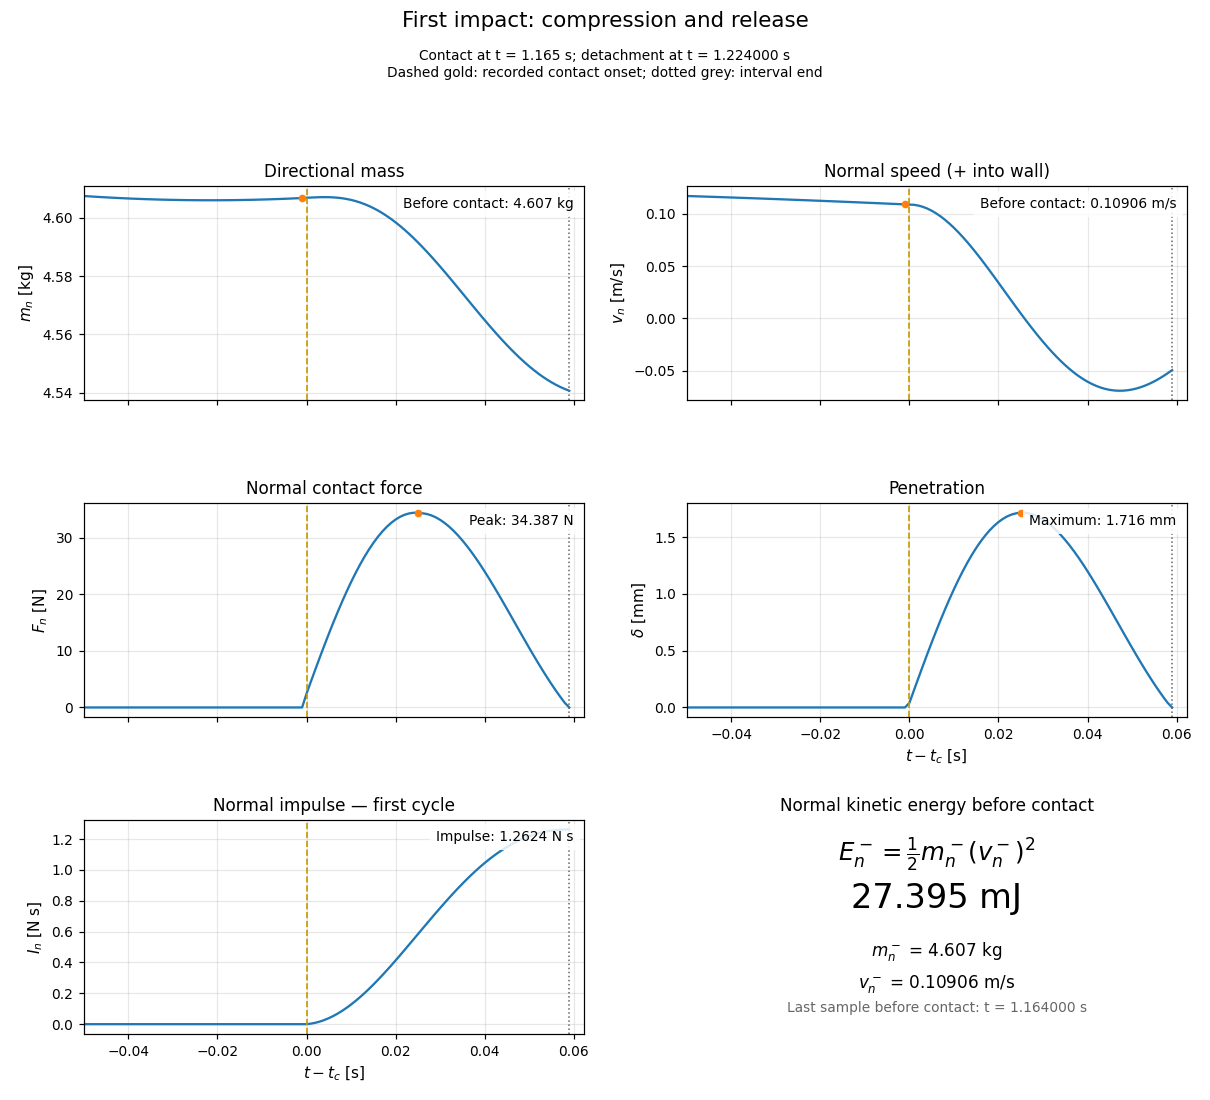
\includegraphics[width=\linewidth]{fig04_circular_online_first_impact}
\caption{Circular full-online controller, first compression--release cycle.}
\label{fig:circular-online-first}
\end{figure}
\begin{figure}[p]
\centering
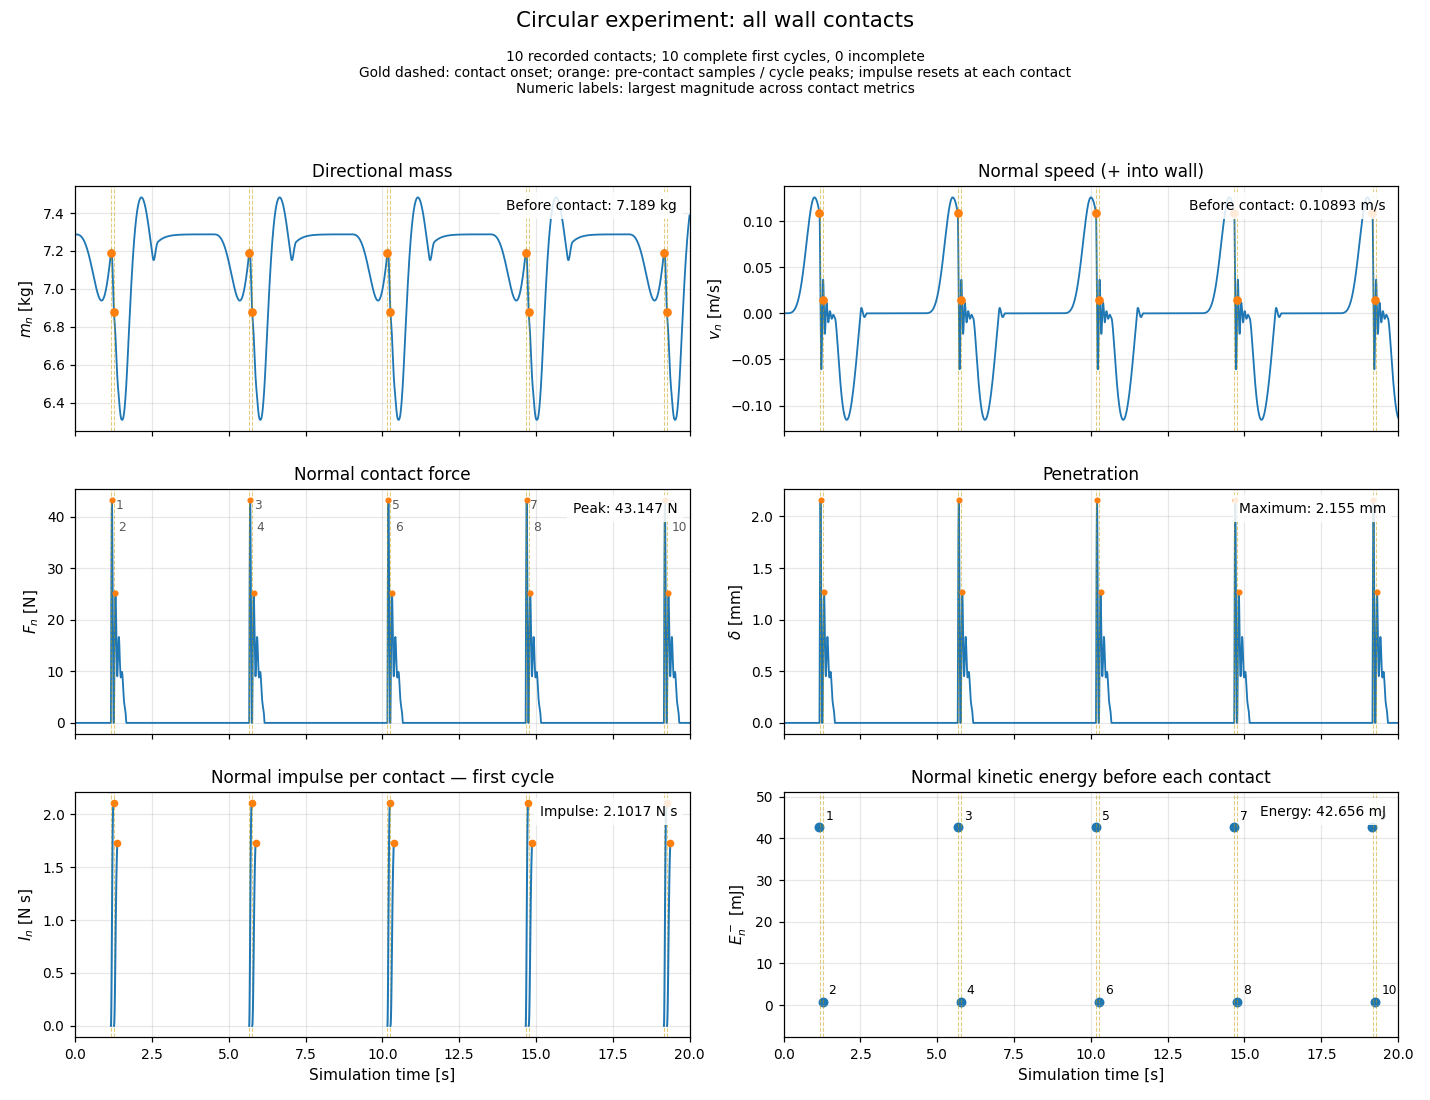
\includegraphics[width=\linewidth]{fig05_circular_baseline_all_collisions}
\caption{Circular baseline, all contacts with the shared return schedule.
Each numeric label selects the largest absolute contact metric over the run.}
\label{fig:circular-baseline-all}
\end{figure}
\begin{figure}[p]
\centering
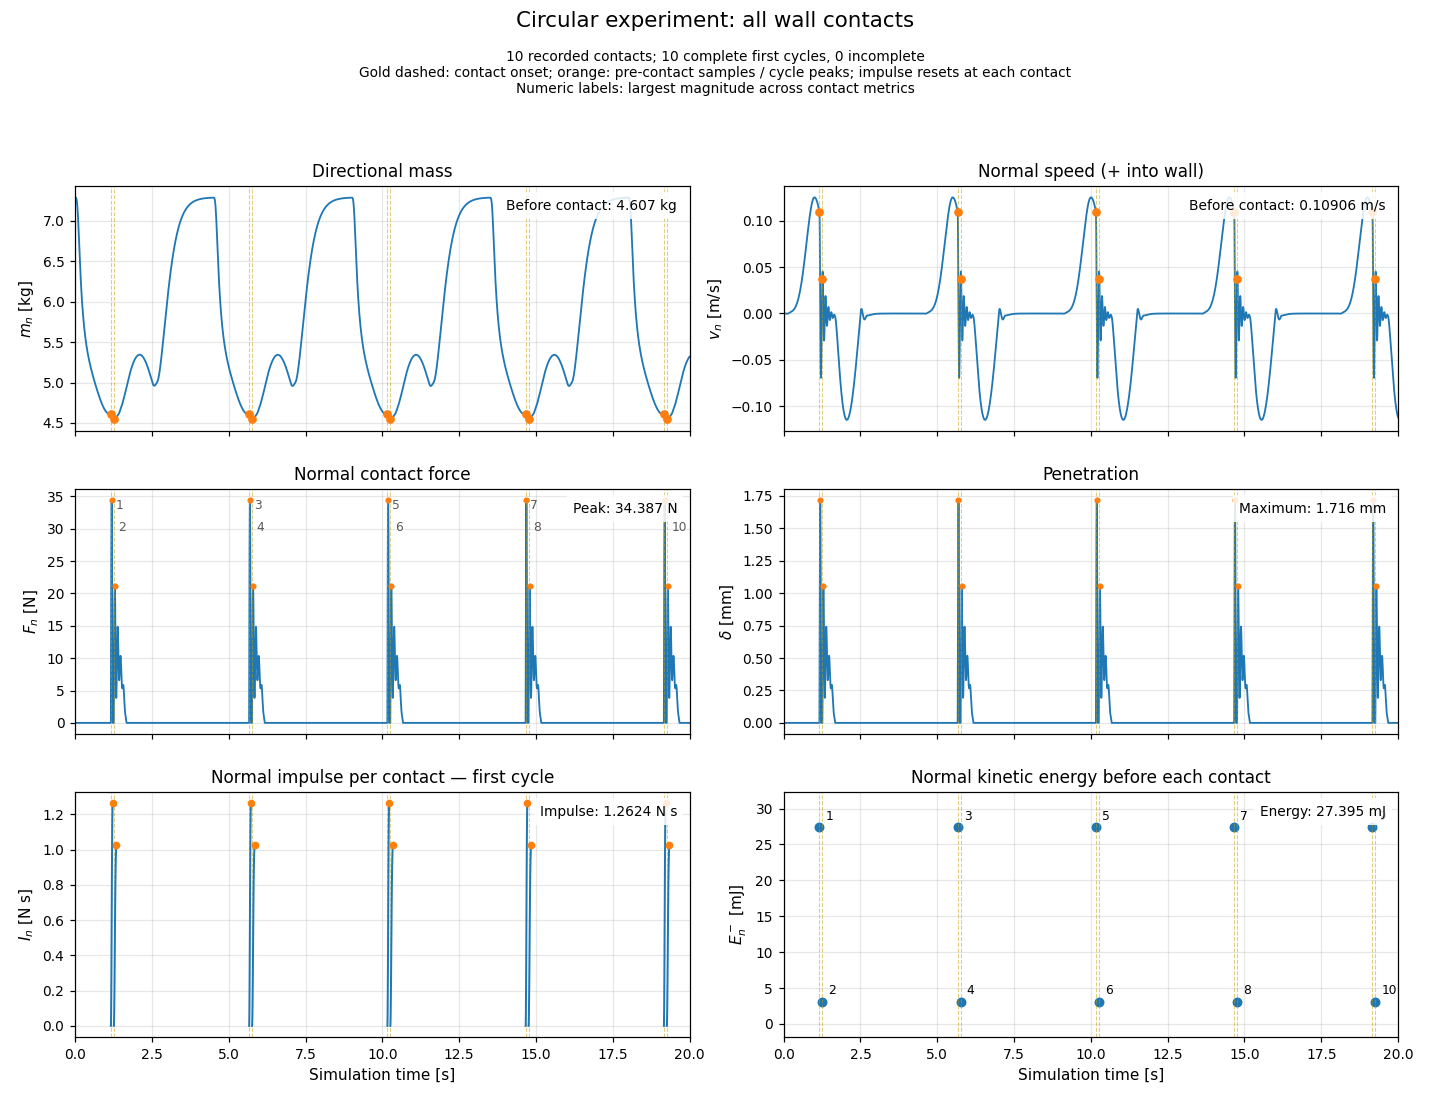
\includegraphics[width=\linewidth]{fig06_circular_online_all_collisions}
\caption{Circular full-online controller, all contacts with the shared return
schedule. Recontacts are included in the labelled contact metrics.}
\label{fig:circular-online-all}
\end{figure}
\clearpage

\subsection{Perpendicular approach}
\begin{table}[htbp]
\centering
\begin{tabular}{lrrr}
\toprule
Metric & Baseline & Full online & Change (\%)\\
\midrule
Contact onset (s) & 0.350 & 0.347 & --\\
Pre-impact effective mass (kg) & 7.622 & 4.908 & $-35.60$\\
Pre-impact normal velocity (m/s) & 0.19969 & 0.20135 & $+0.83$\\
Pre-impact normal energy (mJ) & 151.967 & 99.496 & $-34.53$\\
Peak force (N) & 85.128 & 67.411 & $-20.81$\\
First-cycle impulse (N\,s) & 3.5484 & 2.4579 & $-30.73$\\
Peak penetration (mm) & 4.251 & 3.364 & $-20.88$\\
First-cycle duration (ms) & 64.0 & 55.0 & $-14.06$\\
Pre-impact RMS error (mm) & 0.0656 & 0.3425 & --\\
\bottomrule
\end{tabular}
\caption{First perpendicular compression--release cycle.}
\label{tab:perpendicular}
\end{table}

At approximately 0.20\,m/s, the perpendicular approach tests contact at
almost twice the circular entry speed. Both a lower mean force (44.7\,N
instead of 55.4\,N) and a 9\,ms shorter cycle contribute to the lower
impulse. Peak force and penetration fall by about one fifth, with a
slightly higher entry speed in the online run.

The pre-impact Cartesian RMS error increases by 0.277\,mm. Its absolute
value stays below 0.35\,mm in all four trials, but the increase shows that
the same Cartesian feedback gains can produce different tracking once the
QP bounds are active. Figures~\ref{fig:perpendicular-baseline}
and~\ref{fig:perpendicular-online} show the separate force histories.

\begin{figure}[p]
\centering
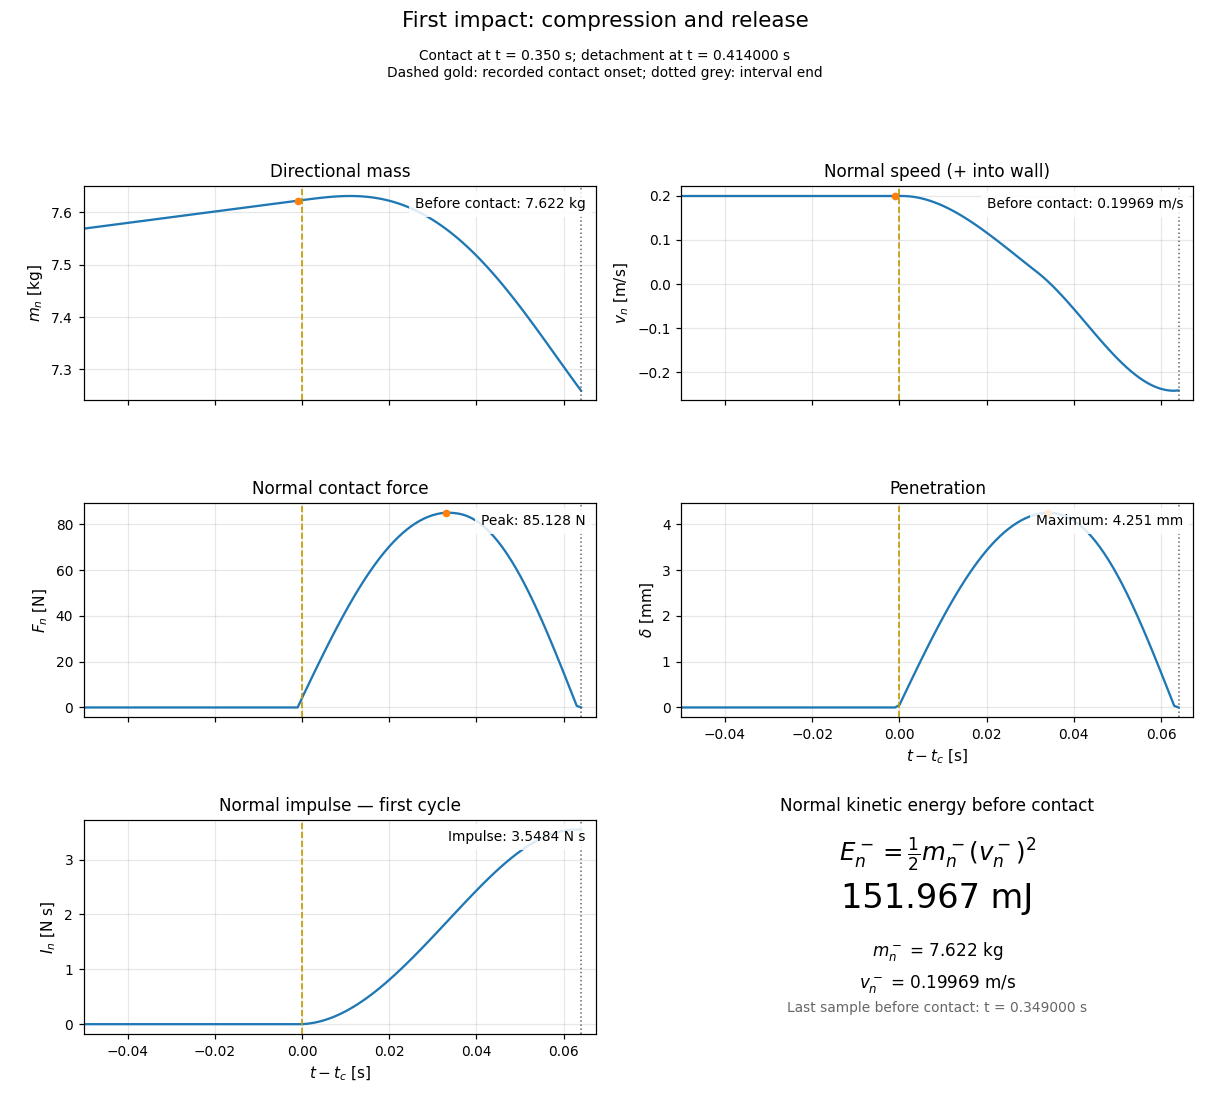
\includegraphics[width=\linewidth]{fig07_perpendicular_baseline_first_impact}
\caption{Perpendicular baseline, first compression--release cycle.}
\label{fig:perpendicular-baseline}
\end{figure}
\begin{figure}[p]
\centering
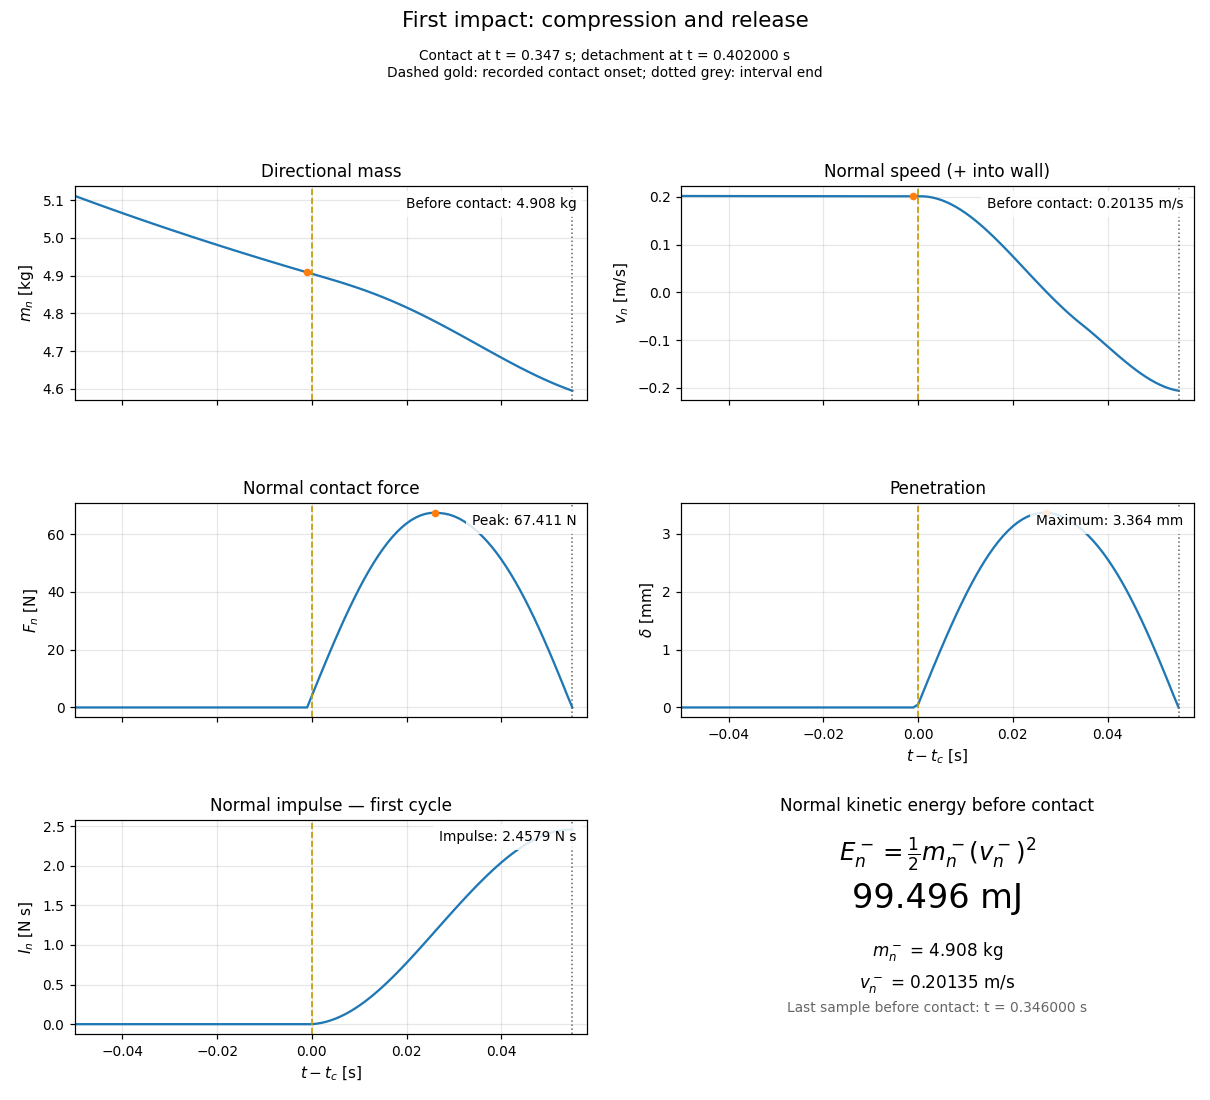
\includegraphics[width=\linewidth]{fig08_perpendicular_online_first_impact}
\caption{Perpendicular full-online controller, first compression--release cycle.}
\label{fig:perpendicular-online}
\end{figure}
\clearpage

\subsection{Interpretation using an elastic impact model}
To relate the measured mass reduction to the contact loads, consider a
constant mass $\ms$ approaching an undamped spring with stiffness $k_e$.
With no actuation during contact, the compression satisfies
\begin{equation}
 \ms\ddot\delta+k_e\delta=0,\qquad
 \delta(0)=0,\quad\dot\delta(0)=\vs .
\end{equation}
Writing $\omega=\sqrt{k_e/\ms}$ gives
$\delta(t)=(\vs/\omega)\sin(\omega t)$. The first release occurs at
$T_{\mathrm{el}}=\pi/\omega$. The peak force and impulse are
\begin{equation}
 F_{\mathrm{peak,el}}=\vs\sqrt{k_e\ms},\qquad
 I_{\mathrm{el}}=2\ms\vs,\qquad
 T_{\mathrm{el}}=\pi\sqrt{\ms/k_e}.
 \label{eq:elastic}
\end{equation}
At equal velocity, a 30\% effective mass reduction predicts a peak-force
reduction of $1-\sqrt{0.70}=16.3\%$ and an impulse reduction of 30\%.
Table~\ref{tab:elastic} evaluates equation~\eqref{eq:elastic} at the
actual pre-impact mass and velocity of each run.

\begin{table}[htbp]
\centering
\small
\setlength{\tabcolsep}{5pt}
\begin{tabular}{lrrrrrr}
\toprule
&\multicolumn{3}{c}{Elastic prediction}&\multicolumn{3}{c}{Simulation}\\
\cmidrule(lr){2-4}\cmidrule(lr){5-7}
Quantity & Baseline & Online & Change (\%) & Baseline & Online & Change (\%)\\
\midrule
\multicolumn{7}{l}{\emph{Circular}}\\
Peak force (N) & 41.31 & 33.10 & $-19.86$ & 43.15 & 34.39 & $-20.30$\\
Impulse (N\,s) & 1.566 & 1.005 & $-35.85$ & 2.102 & 1.262 & $-39.93$\\
Duration (ms) & 59.6 & 47.7 & $-19.95$ & 84.0 & 59.0 & $-29.76$\\
\midrule
\multicolumn{7}{l}{\emph{Perpendicular}}\\
Peak force (N) & 77.97 & 63.09 & $-19.09$ & 85.13 & 67.41 & $-20.81$\\
Impulse (N\,s) & 3.044 & 1.977 & $-35.07$ & 3.548 & 2.458 & $-30.73$\\
Duration (ms) & 61.3 & 49.2 & $-19.75$ & 64.0 & 55.0 & $-14.06$\\
\bottomrule
\end{tabular}
\caption{Elastic predictions and measured first compression--release cycles.}
\label{tab:elastic}
\end{table}

The peak-force reduction agrees with the elastic prediction within 1.8
percentage points in both experiments. The circular duration decreases more
than predicted (29.76\% versus 19.95\%), while the perpendicular duration
decreases less (14.06\% versus 19.75\%). This partly explains the differences
between the predicted and simulated impulse reductions.

The measured impulses are 16.6--34.2\% higher than $2\ms\vs$.
The model omits wall damping, continued control action and changes in
$m_n(q)$ during contact. The wall damping ratio
$b_e/(2\sqrt{k_e\ms})$ is about 0.02. Continued actuation can push the
fingertip toward the wall and may prolong loading. These effects prevent
the passive model from reproducing the complete force history.

\subsection{Collision detection and reconstructed force}
The circular baseline and online runs each produce five rising detection
events, with no off-contact onset. The threshold is crossed 5\,ms after
fingertip contact. Ten force episodes produce five detection events
because the filtered residual can stay above threshold between an impact
and a recontact. In the perpendicular trials, the baseline and online
detections each occur 4\,ms after first contact. These observations describe
the four selected runs. Smooth reference and torque transitions reduce
the abrupt changes that can excite observer transients.

Figures~\ref{fig:observer-circular} and~\ref{fig:observer-perpendicular}
show the detection signals for the online runs.

\begin{figure}[p]
\centering
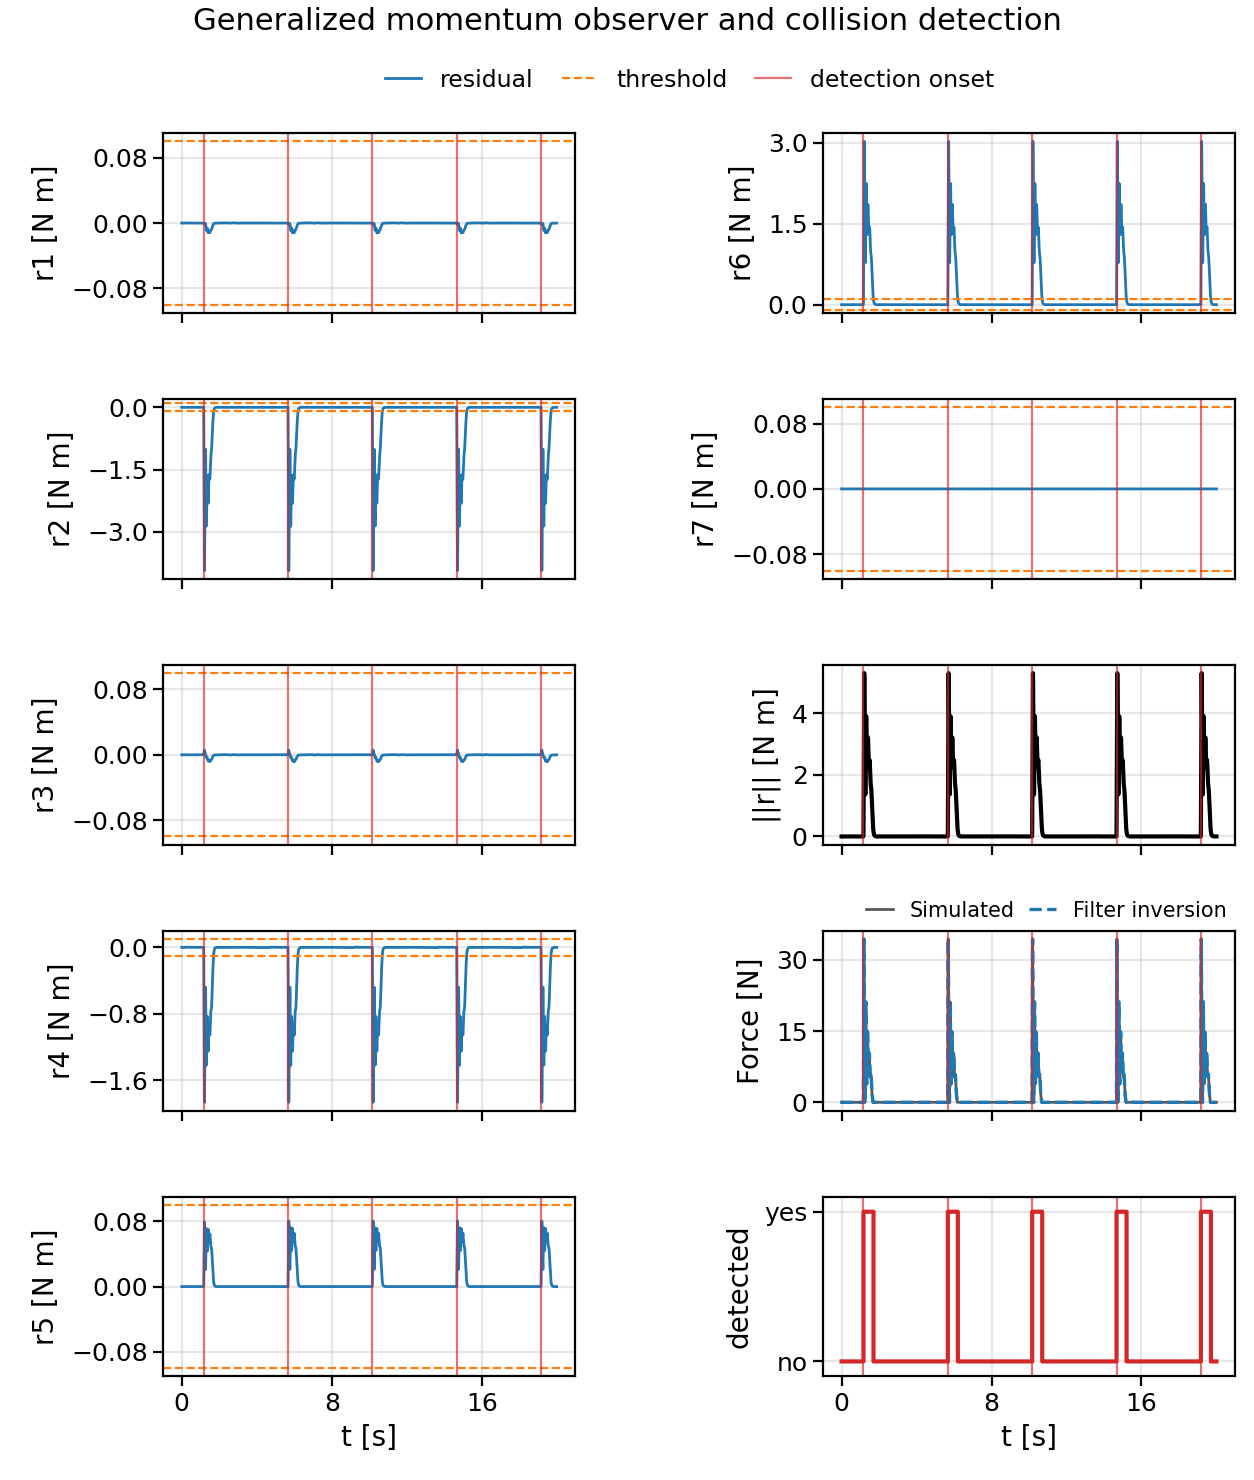
\includegraphics[width=\linewidth,height=0.87\textheight,keepaspectratio]{fig01_observer_qp_circular}
\caption{Observer diagnostic for the circular single-QP run.}
\label{fig:observer-circular}
\end{figure}
\begin{figure}[p]
\centering
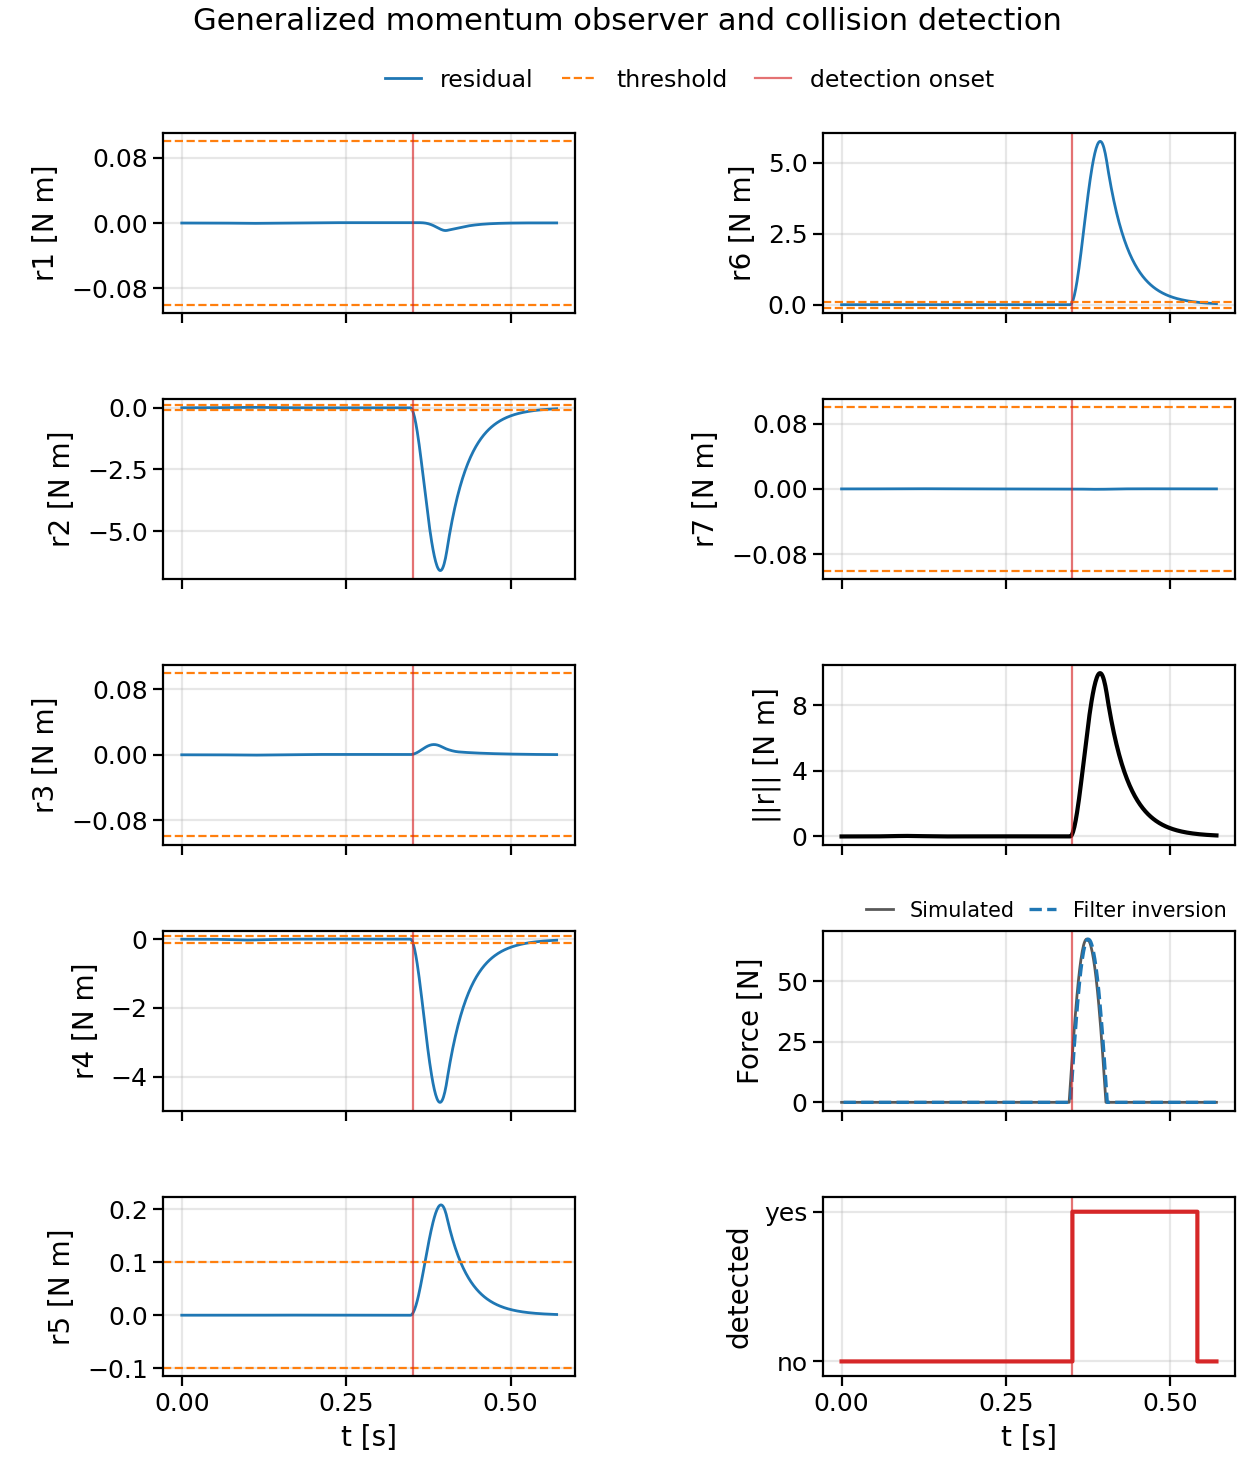
\includegraphics[width=\linewidth,height=0.87\textheight,keepaspectratio]{fig02_observer_qp_perpendicular}
\caption{Observer diagnostic for the perpendicular single-QP run.}
\label{fig:observer-perpendicular}
\end{figure}
\clearpage

At $K_O=30I_7$\,s$^{-1}$, the observer time constant is about 33\,ms.
The online simulated forces peak 25--26\,ms after first contact.
Direct projection of the filtered residual underestimates the peaks
by 43.0\% in the circular run and 42.4\% in the perpendicular run,
with a 20\,ms delay in both. Inverting the discrete filter with
equation~\eqref{eq:force-estimation} brings both peaks within 0.05\,N
of the simulated force and reduces the peak delay to 2\,ms
(Figure~\ref{fig:force}). The derivative in that reconstruction is
sensitive to measurement noise, model errors and timing errors.

\begin{figure}[htbp]
\centering
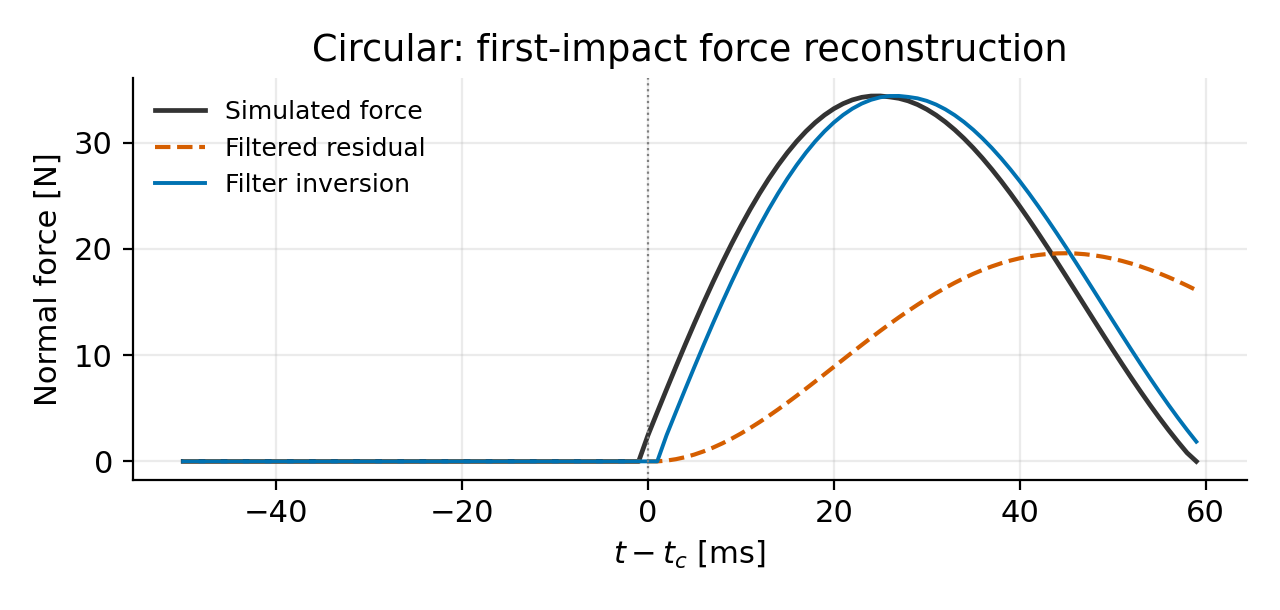
\includegraphics[width=0.94\linewidth]{fig09_force_estimation_circular.png}\par
\medskip
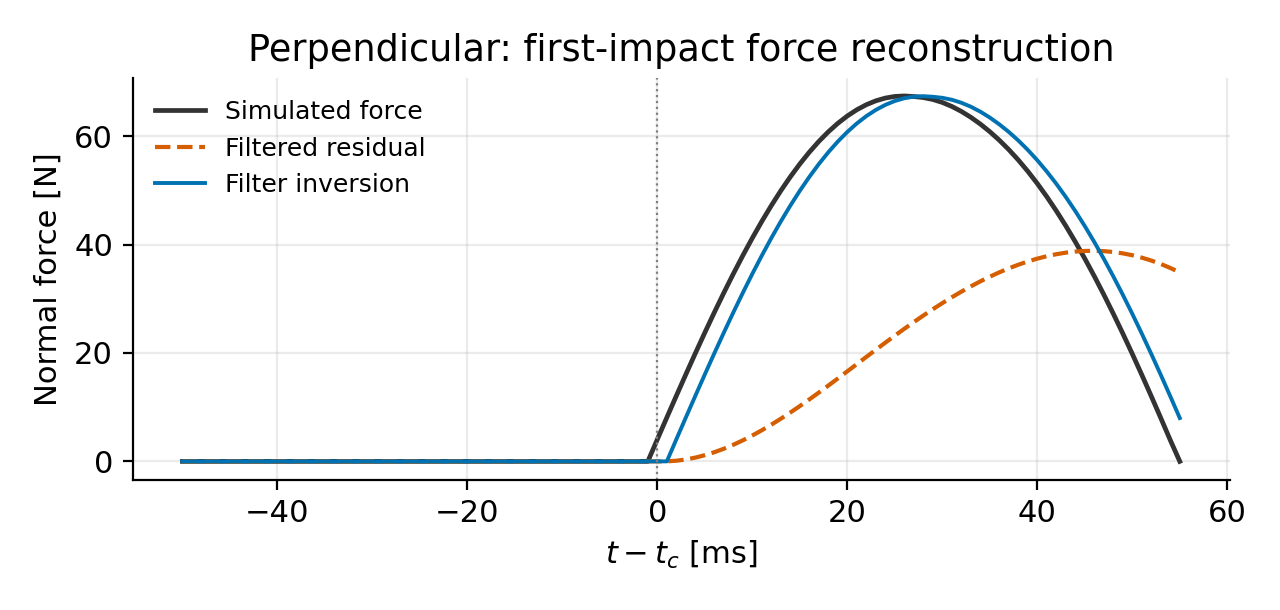
\includegraphics[width=0.94\linewidth]{fig10_force_estimation_perpendicular.png}
\caption{Simulated and reconstructed normal force during the first
circular (top) and perpendicular (bottom) online impacts.}
\label{fig:force}
\end{figure}
\clearpage

\subsection{Constraint checks and computation}
\begin{table}[htbp]
\centering
\small
\begin{tabular}{lrrrr}
\toprule
Online run & QP updates & Rejected & Min.\ margin (rad) & Peak motor limit (\%)\\
\midrule
Circular & 19998 & 0 & 0.12450 & 47.3\\
Perpendicular & 569 & 0 & 0.06889 & 77.8\\
\bottomrule
\end{tabular}
\caption{QP acceptance, minimum sampled joint clearance and peak
nominal motor torque as a percentage of its configured limit.}
\label{tab:qp}
\end{table}

Both online trials complete with every QP solution accepted. The
maximum recorded inequality errors are $2.91\times10^{-5}$ and
$4.40\times10^{-5}$ for the circular and perpendicular trials,
respectively. Both are within the numerical acceptance tolerance.
No samples exceed the configured hard position, velocity or torque
limits, and there is no actuator clipping. The circular motion enters
the braking buffer. The perpendicular trial approaches within
0.009\,rad of its hard position margin, leaving less clearance for
perturbations. Both pairs pass the comparison tool's first-impact
and sampled-limit criteria.

\begin{table}[htbp]
\centering
\small
\setlength{\tabcolsep}{5pt}
\begin{tabular}{lrrrrr}
\toprule
Run & \shortstack{Update mean\\(ms)} & \shortstack{Update p95\\(ms)}
& \shortstack{Update max.\\(ms)} & \shortstack{Callback p95\\(ms)}
& \shortstack{Missed samples\\count (\%)}\\
\midrule
Circular baseline & 0.498 & 0.900 & 17.102 & 1.672 & 3 (0.015)\\
Circular online & 0.591 & 0.964 & 10.748 & 1.714 & 3 (0.015)\\
Perpendicular baseline & 0.448 & 0.628 & 10.687 & 1.413 & 1 (0.175)\\
Perpendicular online & 0.508 & 0.876 & 10.105 & 1.601 & 2 (0.350)\\
\bottomrule
\end{tabular}
\caption{Wall-clock timing for controller updates and simulator callbacks.
p95 denotes the 95th percentile.}
\label{tab:timing}
\end{table}

The online update p95 values are below the 1\,ms period of a 1\,kHz
loop. The full simulator callback includes controller execution,
monitoring and publication, and its p95 exceeds 1\,ms in both trials.
The update maxima exceed even the 5\,ms budget at RTF 0.20. These
measurements characterize the simulator and show why a separate
end-to-end timing test is needed for real-time operation.

\section{Discussion and limits}
Both experiments meet the effective mass target with pre-impact speeds
within 1\% of their baselines. The QP controller achieves lower contact
loads with larger pre-impact position errors. The two implementations
also differ in their pseudoinverse, redundant-motion damping and constraint
handling. An ablation study with matched redundancy and constraints would
help isolate the contribution of the mass gradient.

Earlier variants explored attraction to a fixed low-mass posture computed
offline and a separate contact phase with impedance feedback. The first
required an additional posture optimization for each task, while the
second changed the Cartesian law during contact. The current optimization
uses the online mass gradient and one tracking law throughout each approach.

The main geometric limitation is the fingertip contact assumption. In the
online runs, the hand bounding-box diagnostic first overlaps the wall plane
29\,ms before circular fingertip contact and 15\,ms before perpendicular
contact. Its maximum overlap is 5.40 and 7.08\,mm, respectively. The virtual
wall applies force at the fingertip.

On hardware the hand could touch first, changing the contact Jacobian and
the effective mass relevant to the collision. A simulation with hand and link
contacts would help determine whether the low-mass postures leave enough
clearance. Adding orientation or clearance constraints would reduce the set
of available postures.

The braking bounds use nominal accelerations from the actuator command.
An external force can change the joint motion during impact. Sampled-limit
compliance in the two trials leaves open the effect of model errors, friction,
sensor noise and missed updates. Those perturbations also affect the observer.
In particular, the derivative used for force reconstruction amplifies changes
in the residual.

\section{Conclusions}
A single weighted QP reduced pre-impact effective mass by 35.92\% on the
circular trajectory and by 35.60\% in the perpendicular approach. At nearly
equal entry speeds, peak forces fell by 20.30\% and 20.81\%, and first-cycle
impulses fell by 39.93\% and 30.73\%, respectively. The pre-impact tracking
error increased in both experiments while remaining below 0.35\,mm RMS.

A passive elastic model explains the approximate scaling of the peak force.
The measured duration and impulse reflect the force history during controlled
contact. A shared physical return to the initial posture aligns successive
circular approaches and prevents joint posture from accumulating across laps.

The next steps toward the Franka Emika R3 are to check potential hand
contact, test the joint braking and force reconstruction under realistic
perturbations, and measure end-to-end execution at 1\,kHz. The observed
callback timing and joint clearances make those checks relevant even though
the four nominal trials completed.

\clearpage
\appendix
\section{Recorded data sources}
\label{app:sources}
Paths are relative to the \texttt{fr3\_student\_sim} directory. All four
runs use a requested RTF of 0.20 with the observer enabled.

\begin{itemize}
\item Circular baseline:
  \path{runs/circle_baseline_20261127_095345.npz}
\item Circular online:
  \path{runs/optimized_full_online_qp_circular_20261127_094742.npz}
\item Perpendicular baseline:
  \path{runs/baseline_perp_20261127_095738.npz}
\item Perpendicular online:
  \path{runs/report_qp_20261127/optimized_full_online_qp_perp_report_20261127_100638.npz}
\end{itemize}
The perpendicular online source is the dedicated run with collision
monitoring enabled. All plots were generated by the project's
\texttt{plot\_run} executable using the listed files. The force-reconstruction
figures use the two online logs. All first-impact and timing tables use the
same recorded pairs.

\clearpage

\begin{thebibliography}{9}
\phantomsection
\addcontentsline{toc}{section}{References}
\bibitem{khatib1987}
O.~Khatib, \emph{A unified approach for motion and force control of robot
manipulators: The operational space formulation}, IEEE Journal
on Robotics and Automation, vol.~3, no.~1, pp.~43--53, 1987.
\bibitem{haddadin2017}
S.~Haddadin, A.~De~Luca, and A.~Albu-Sch\"affer, \emph{Robot collisions:
A survey on detection, isolation, and identification}, IEEE
Transactions on Robotics, vol.~33, no.~6, pp.~1292--1312, 2017.
\bibitem{deluca2005}
A.~De~Luca and R.~Mattone, \emph{Sensorless robot collision detection and
hybrid force/motion control}, Proc. IEEE Int. Conf. on Robotics
and Automation (ICRA), 2005, pp.~999--1004.
\bibitem{franka-fci}
Franka Robotics, \emph{libfranka Overview}, Franka Control Interface
documentation. \url{https://frankarobotics.github.io/docs/doc/libfranka/docs/overview.html}.
\end{thebibliography}
\end{document}
